
\section{Predspracovanie obrazu}

%http://scikit-image.org/docs/dev/auto\_examples/
% Normalizacia obrazu - github ten kurz c231n - 17150\_FULLTEXT.pdf (normalization)
%\subsection{Hogova transformacia}
% - F3-DP-2016-Erlebach-Jonas-Automaticka detekce pupily v obraze.pdf
%\subsection{Detekcia hran}
%- Sobelov filter - podľa knižky patri medzi najpopulárnejšie hranové filter. Urobiť z neho magnitúdu obrazu potom.

% Nieco na sposob ze, kedze riesenie bude obsahovat aj klasicke pristupy nie len riesenie s pouzitim
% neurovnovych sieti, je dolezite obrazky pred klasifikaciou vhodne upravit resp. extrahovat z obrazku vhodne priznaky na zaklade
% ktorych sa klasifikator bude ucit.

\subsubsection{Rovnomerný pomer strán}
Pre spracovanie obrázkov pomocou neurónových sieti je potrebné zabezpečiť, aby každý obrázok mal rovnakú veľkosť a rovnaký pomer strán.
Väčšina modelov neurónovej siete predpokladá štvorcový vstupný obraz \cite{odkaz:NNPreprocessing}.

\subsubsection{Priemerna štandartná odchylka vstupných údajov}
Je užitočné vytvoriť si tzv. ''stredný obraz'' získaný priemernými hodnotami pre každý pixel zo všetkých trénovacích dát.
Timto spôsobom je možné vytvoriť si základny prehľad o štruktúre vstupných dát.
Na základe toho môžeme potom do vstupným dát pridať rôzne dalšie variácie klasifikovaných objektov pre lepšie generalizovanie klasifikátora \cite{odkaz:NNPreprocessing}.

\subsubsection{Šedotónový obraz}
Ďalšou možnou technikou je vytvorenie šedotónového obrazu, kde všetky 3 zložky farby (RGB) zlúčime do jednej, šedotónovéj.
\begin{figure}[H]
	\centering
	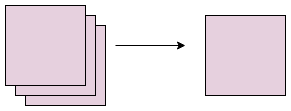
\includegraphics[width=0.4\textwidth]{grayscale}
	\caption{Prevod do šedotónového obrazu[eng. grayscaling]\cite{odkaz:NNPreprocessing}}
	\label{pic:GrayScaling}
\end{figure}

\subsubsection{Rožšírenie vstupných dát}
Ďalšou bežnou technickou predspracovanie dát je rožšírenie existujúceho súboru dát s rôznymi variáciami existujúcich obrázkov.
Tieto variácie môžu zahŕňať zväčšovanie, zmenšovanie, rotačné zmeny a iné transformácie obrázkov.
Tento postup znižuje šancu, že neurónová sieť rozpozná nežiadúce charakteristiky v množine vstupných dát \cite{odkaz:NNPreprocessing}.
